%%%%%%%%%%%%%%%%%%%%%%%%%%%%%%%%%%%%%%%%%
% Beamer Presentation
% LaTeX Template
% Version 1.0 (10/11/12)
%
% This template has been downloaded from:
% http://www.LaTeXTemplates.com
%
% License:
% CC BY-NC-SA 3.0 (http://creativecommons.org/licenses/by-nc-sa/3.0/)
%
%%%%%%%%%%%%%%%%%%%%%%%%%%%%%%%%%%%%%%%%%

%----------------------------------------------------------------------------------------
%	PACKAGES AND THEMES
%----------------------------------------------------------------------------------------

\documentclass[14pt]{beamer}

\mode<presentation> {

% The Beamer class slide themes
\usetheme{Madrid} %i was using this one

% Beamer class color themes

%\usecolortheme{albatross}

%\setbeamertemplate{footline} % To remove the footer line in all slides uncomment this line
%\setbeamertemplate{footline}[page number] % To replace the footer line in all slides with a simple slide count uncomment this line

%\setbeamertemplate{navigation symbols}{} % To remove the navigation symbols from the bottom of all slides uncomment this line
}

\usepackage{graphicx} % Allows including images
\usepackage{booktabs} % Allows the use of \toprule, \midrule and \bottomrule in tables
\usepackage{hyperref}
\usepackage{helvet}

%----------------------------------------------------------------------------------------
%	TITLE PAGE
%----------------------------------------------------------------------------------------

\title[Intro to R]{Introduction to R} % The short title appears at the bottom of every slide, the full title is only on the title page

\author{C. Ryan Campbell} % Your name
\institute[Duke] % Your institution as it will appear on the bottom of every slide, may be shorthand to save space
{
Duke University \\ % Your institution for the title page
\medskip
\textit{c.ryan.campbell@duke.edu} % Your email address
}
\date{07 Sept 2017} % Date, can be changed to a custom date

\begin{document}

\begin{frame}
\titlepage % Print the title page as the first slide
\end{frame}

\begin{frame}
\frametitle{Overview} % Table of contents slide, comment this block out to remove it
\tableofcontents % Throughout your presentation, if you choose to use \section{} and \subsection{} commands, these will automatically be printed on this slide as an overview of your presentation
\end{frame}

%----------------------------------------------------------------------------------------
%	PRESENTATION SLIDES
%----------------------------------------------------------------------------------------

%------------------------------------------------
\section{Intro} % Sections can be created in order to organize your presentation into discrete blocks, all sections and subsections are automatically printed in the table of contents as an overview of the talk
%------------------------------------------------

%------------------------------------------------
\begin{frame}
\frametitle{Software-Based Labs}
%what students should know/learn today
\begin{itemize}
	\item<+-> R
	\begin{itemize}
		\item Already have all the software needed
	\end{itemize}
	\item<+-> bin/bash
	\begin{itemize}
		\item Waiting for cluster access
		\item Next week (fingers crossed)
	\end{itemize}
	\item<+-> git
	\begin{itemize}
		\item Best to wait for groups to be formed
		\item Next week as well (fingers crossed)
	\end{itemize}
\end{itemize}
\end{frame}

%------------------------------------------------
\begin{frame}
\frametitle{Software-Based Labs}
\begin{itemize}
	\item<+-> Take a minute to download a text editor
	\begin{itemize}
		\item TextEdit
		\item Sublime
		\item TextWrangler
		\item Notepad++
	\end{itemize}
	\item<+-> Work along with the slides (in R-Studio or an editor), generating a document to test each command
	\item<+-> I'll upload my finished document after class as a reference
\end{itemize}
\end{frame}

%------------------------------------------------
\section{Goals} % A subsection can be created just before a set of slides with a common theme to further break down your presentation into chunks
%------------------------------------------------

%------------------------------------------------
\begin{frame}
\frametitle{Today's Goals}
\begin{itemize}
	\item Get familiarized with R basics
	\item Import your own data
	\item Visualize it
	\item Test something about it
	\item Produce a graph and save the code
\end{itemize}
\end{frame}

%------------------------------------------------
\section{R Basics}
%------------------------------------------------

%------------------------------------------------
\subsection{Variables}
%------------------------------------------------

%------------------------------------------------
\begin{frame}
\frametitle{Variables}
\begin{itemize}
	\item Notes and tips go here
	\item Descriptions of actions not meant to be typed
	\ttfamily
	\begin{block}{}
		\item[] within these boxes will be typed into R
		\item[] it will also have monospaced font
		\item[] > it may also begin with a carat character,
		\item[] which symbolizes the prompt
		\item[] \textit{when it is italicized, it is output from R}
	\end{block}
	\sffamily
\end{itemize}
\end{frame}

%------------------------------------------------
\begin{frame}
\frametitle{Variables}
\begin{itemize}
	\item Scalars, Vectors, Data Frames
	\item Access parts of each with brackets:
	\ttfamily
	\begin{block}{}
		\item[] > a <- c(15,12,10,93)
		\item[] > a[2]
		\item[] \textit{ 12}
	\end{block}
	\sffamily
\end{itemize}
\end{frame}

%------------------------------------------------
\begin{frame}
\frametitle{Variables}
\begin{itemize}
	\item or multiple parts at once with a second vector
	\ttfamily
	\begin{block}{}
		\item[] > a <- c(15,12,10,93)
		\item[] > a[c(2,4)]
		\item[] \textit{ 12 93}
	\end{block}
	\sffamily
\end{itemize}
\end{frame}

%------------------------------------------------
\begin{frame}
\frametitle{Variables}
\begin{itemize}
	\item or with a TRUE/FALSE vector
	\ttfamily
	\begin{block}{}
		\item[] > a <- c(15,12,10,93)
		\item[] > a[c(FALSE,TRUE,TRUE,FALSE)]
		\item[] \textit{ 12 93}
	\end{block}
	\sffamily
\end{itemize}
\end{frame}

%------------------------------------------------
\begin{frame}
\frametitle{Variables \& Math}
\begin{itemize}
	\item Scalar mathematical operations apply to an entire vector
	\ttfamily
	\begin{block}{}
		\item[] > a * 5
		\item[] \textit{  75  60  50 465}
	\end{block}
	\sffamily
\end{itemize}
\end{frame}

%------------------------------------------------
\begin{frame}
\frametitle{Variables \& Math}
\begin{itemize}
	\item Vector mathematical operations apply to each entry
	\ttfamily
	\begin{block}{}
		\item[] > a + c(1,1,10,-50)
		\item[] \textit{  16 13 20 43}
	\end{block}
	\sffamily
	\item This is useful because it allows you to manipulate entire sets of data at once
	\begin{itemize}
		\item Take the absolute value of a column
		\item Combine columns to create new measures
		\item Plot the log(value) of a dataset instead of the raw value
	\end{itemize}
\end{itemize}
\end{frame}

%------------------------------------------------
\subsection{Data Frames \& Matrices}
%------------------------------------------------

%------------------------------------------------
\begin{frame}
\frametitle{Data Frames and Matrices}
\begin{itemize}
	\item Used to hold data
	\item Can keep track of large sets of data
	\item Like the data from the hypoxia example
\end{itemize}
\end{frame}

%------------------------------------------------
\begin{frame}
\frametitle{Data Frames and Matrices}
\begin{itemize}
	\item Can also be accessed with brackets []
	\begin{itemize}
		\item Brackets require 2 entries instead of 1
		\item because the data has two dimensions
	\end{itemize}
	\item dataframe[row,column]
	\item For example, access a column of the data with brackets:
	\ttfamily
	\begin{block}{}
		\item[] > hypoxiaTested[,1]
		\item[] \textit{[1] TIMM TIMM TIMM TIMM TIMM}
	\end{block}
	\sffamily
	\item (leaving either row or column blank returns the entire range)
\end{itemize}
\end{frame}

%------------------------------------------------
\subsection{Functions}
%------------------------------------------------

%------------------------------------------------
\begin{frame}
\frametitle{Functions}
\begin{itemize}
	\item<+-> Things you do to/with variables
	\item<+-> Are filled with arguments
	\item<+-> Examples:
	\begin{itemize}
		\item<+-> plot()
		\item<+-> ttest()
		\item<+-> read.table()
	\end{itemize}
	\item<+-> What are the arguments for these functions?
	\item<+-> How would you go about answering this question?
	%%UNCOMMENT
	\begin{itemize}
		\item<+-> type ?read.table
		\item<+-> begin typing ``read.table('' and press ``TAB''
	\end{itemize}
\end{itemize}
\end{frame}

%------------------------------------------------
\begin{frame}
\frametitle{?read.table}
\begin{figure}
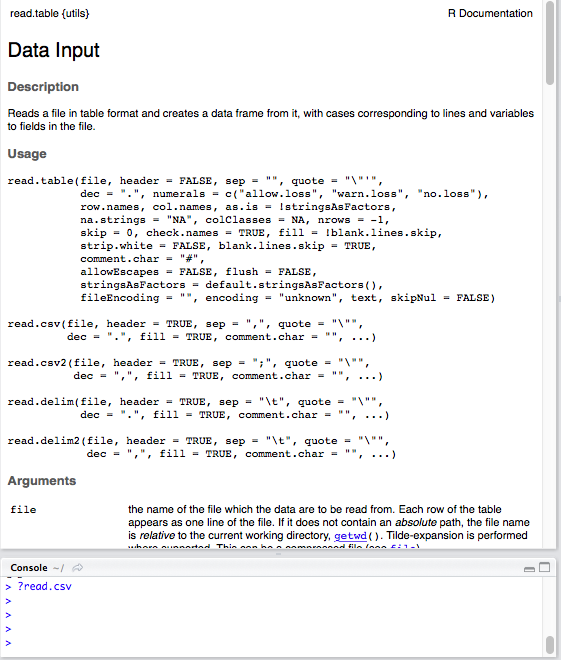
\includegraphics[width=0.52\linewidth]{images_20170907_readcsv.png}
\end{figure}
\end{frame}

%------------------------------------------------
\subsection{Reading in Data}
%------------------------------------------------

%------------------------------------------------
\begin{frame}
\frametitle{Reading in Data}
\begin{itemize}
	\item What are the (relevant) arguments of read.table?
	\begin{itemize}
		\item<+-> file - name of file to bring in, can include location
		\begin{itemize}
			\item ``filename.txt'' or ``/Users/ryan/Documents/filename.txt''
		\end{itemize}
		\item<+-> header - T/F variable to treat the first row like a header
		\item<+-> dec - what character represents decimals
	\end{itemize}
	\begin{block}{}<+->
		\footnotesize
		\item[] \texttt{ > read.table(``hsap\_hypoxia\_gene\_exp\_FORCLASS.diff'',}
		\item[] \texttt{header = TRUE, dec = ``.'')}
		\item[] \texttt{\textit{gene\_family sample\_1 sample\_2...}}
		\item[] \texttt{\textit{1           TIMM     hypo     norm...}}
	\end{block}
\end{itemize}
\end{frame}

%------------------------------------------------
\begin{frame}
\frametitle{Reading in Data}
\begin{itemize}
	\item You can store the data as a variable in R
	\begin{itemize}
		\item<1-> This allows for easier manipulation
		\item<2-> Be sure to name it appropriately
		\item<3-> Variable names are usually all letters
		\item<3-> Capitalization can help split up words (e.g. hypoxiaTested, hypoxiaTIMM)
	\end{itemize}
	\begin{block}{}<4->
		\scriptsize
		\item[] \texttt{ > hypoxiaRAW <- read.table(``hsap\_hypoxia\_gene\_exp\_FORCLASS.diff'',}
		\item[] \texttt{header = TRUE, dec = ``.'')}
	\end{block}
	\begin{itemize}
		\item<5-> Was there output from the command? Why or why not?
	\end{itemize}
\end{itemize}
\end{frame}

%------------------------------------------------
\begin{frame}
\frametitle{Data Frames \& Matrices}
\begin{itemize}
	\item In addition to brackets to access parts of a data frame you can also use the \$ in combination with the column name:
	\ttfamily
	\begin{block}{}
		\item[] > hypoxiaTested\$gene\_family
		\item[] \textit{[1] TIMM TIMM TIMM TIMM TIMM}
	\end{block}
	\sffamily
	\item Gives the same as using [,1] next to hypoxiaTested
	\item However it has several advantages
	\begin{itemize}
		\item Clearer in code, so you recognize it later
		\item You can use the TAB key to pick a column name within R-Studio
	\end{itemize}
\end{itemize}
\end{frame}

%------------------------------------------------
\begin{frame}
\frametitle{Data Frames \& Matrices}
\begin{itemize}
	\item Another useful way to use the \$ is to add new data to an existing data frame
	\item Simply generate data and define it as a new column name:
	\ttfamily
	\footnotesize
	\begin{block}{}
		\item[] > hypoxiaTested\$r\_value <- ( hypoxiaTested\$p\_value + hypoxiaTested\$q\_value ) / 2 
	\end{block}
	\sffamily
	\normalsize
	\item What variables did I manipulate?
	\item What is the new ``r value'' column I created?
\end{itemize}
\end{frame}

%------------------------------------------------
\begin{frame}
\frametitle{Visualize the Data}
\begin{itemize}
	\item<+-> You can use functions to see what the data look like:
	\begin{itemize}
		\item<+-> Histograms (hist) can show you what a single variable looks like
		\item<+-> Scatterplots (plot) can show you how variables relate
	\end{itemize}
\end{itemize}
\end{frame}

%------------------------------------------------
\subsection{T-Test}
%------------------------------------------------

%------------------------------------------------
\begin{frame}
\frametitle{A Simple T-Test}
\begin{itemize}
	\item To conduct a simple T-Test I'm going to generate some random, normal data:
	\begin{itemize}
		\footnotesize
		\item (pick your own values for the n and mean to fill out the class chart)
	\end{itemize}
	\ttfamily
	\begin{block}{}
		\item[] > meanzero <- rnorm(100,0,1)
		\item[] > meanthree <- rnorm(100,3,1)
	\end{block}
	\sffamily
	\normalsize
	\item How would I confirm that this data is normally distributed?
\end{itemize}
\end{frame}

%------------------------------------------------
\begin{frame}
\frametitle{A Simple T-Test}
\begin{itemize}
	\item To conduct a simple T-Test I'm going to generate some random, normal data:
	\begin{itemize}
		\footnotesize
		\item (pick your own values for the n and mean to fill out the class chart)
	\end{itemize}
	\ttfamily
	\begin{block}{}
		\item[] > meanzero <- rnorm(100,0,1)
		\item[] > meanthree <- rnorm(100,3,1)
	\end{block}
	\sffamily
	\normalsize
	\item How would I confirm that this data is normally distributed?
	%%UNCOMMENT
	\ttfamily
	\footnotesize
	\begin{block}{}
		\item[] > hist(meanzero, xlim = c(-3,6))
		\item[] > hist(meanthree, add = T, col = "gray")
	\end{block}
\end{itemize}
\end{frame}

%------------------------------------------------
\begin{frame}
\frametitle{A Simple T-Test}
\begin{itemize}
	\item To conduct a simple T-Test use the t.test() function
	\ttfamily
	\footnotesize
	\begin{block}{}
		\item[] > t.test(meanzero,meanthree,var.equal = T)
		\item[] \textit{	Two Sample t-test}
		\item[] \textit{data:  meanzero and meanthree}
		\item[] \textit{t = -21.004, df = 198, p-value < 2.2e-16}
	\end{block}
\end{itemize}
\end{frame}

%------------------------------------------------
\subsection{Exercise}
%------------------------------------------------

%------------------------------------------------
\begin{frame}
\frametitle{Bring in your own Data}
\begin{itemize}
	\item Pick some data from the github
	\item Bring it into a session of R
	\item Make sure the column names are correct
	\item Make sure R interprets numbers correctly
	\begin{itemize}
		\item What do I mean by this?
		\item How does one do this?
	\end{itemize}
\end{itemize}
\end{frame}

%------------------------------------------------
\begin{frame}
\frametitle{Bring in your own Data}
\begin{itemize}
	\item Pick some data from the github
	\begin{itemize}
		\item Biology Data:
		\begin{itemize}
			\item hsap\_hypoxia\_gene\_exp\_FORCLASS.diff
		\end{itemize}
		\item Political Data:
		\begin{itemize}
			\item 2008to2016PresElections.csv
		\end{itemize}
		\item Movie Data:
		\begin{itemize}
			\item movie\_metadata\_genre\_FORCLASS.csv
		\end{itemize}
		\item Sports Data: 
		\begin{itemize}
			\item NCAA\_BBall\_KenPom\_summary17.csv
			\item NFL\_game\_scores.csv, Game\_Logs\_Quarterback.csv, Career\_Stats\_Passing.csv
		\end{itemize}
	\end{itemize}
	\item or \href{https://www.kaggle.com/}{Choose your own!}
\end{itemize}
\end{frame}

%------------------------------------------------
\begin{frame}
\frametitle{Visualize the Data}
\begin{itemize}
	\item<+-> Use the functions hist or plot to explore your data
	\begin{itemize}
		\item<+-> Histograms (hist) can show you what a single variable looks like
		\item<+-> Scatterplots (plot) can show you how variables relate
	\end{itemize}
	\item<+-> Take notes on it within your Rmd session (e.g. status1 is experimental condition, value2 is numeric and ranges from...)
	\item<+-> Plot different variables against each other to see how they relate
	\item<+-> Decide on a pair of variables to test with a \href{https://en.wikipedia.org/wiki/T-test}{T-Test}
\end{itemize}
\end{frame}

%------------------------------------------------
\begin{frame}
\frametitle{Test the Data}
\begin{itemize}
	\item<+-> Make a hypothesis about two subsets of your data
	\item<+-> Use a T-Test to look for differences in two sets of your data
	\item<+-> Add a plot to show the T-Test results
\end{itemize}
\end{frame}

%------------------------------------------------
\begin{frame}
\frametitle{Assignment - Due 9/14}
\begin{itemize}
	\item Import a dataset
	\item Create two subsets
	\item Make a hypothesis about them
	\item Compare the subsets with T-Test
	\item Visualize the results
	\begin{block}{Turn In}
		\item[] - your .Rmd file
		\item[] - your data file
	\end{block}
	\item So that when I run the .Rmd I see your output
\end{itemize}
\end{frame}

%------------------------------------------------
\begin{frame}
\Huge{\centerline{The End}}
\end{frame}

%----------------------------------------------------------------------------------------

\end{document} 